\documentclass[11pt]{article}
% Preamble for a minimal theoretical CS / graph theory style
\usepackage[T1]{fontenc}
\usepackage[utf8]{inputenc}
\usepackage{lmodern}
\usepackage{microtype}

\usepackage{amsmath,amssymb,amsthm,mathtools}
\usepackage{geometry}
\usepackage{hyperref}

\geometry{margin=1in}

% \setlength{\parindent}{0pt}
% \setlength{\parskip}{0.4em}

\hypersetup{
  colorlinks=true,
  linkcolor=black,
  citecolor=black,
  urlcolor=black
}




\usepackage{physics}
\usepackage[shortlabels]{enumitem}
\usepackage{wrapfig, float}
\usepackage{tikz}
\usetikzlibrary{calc}
\usetikzlibrary{positioning, shapes.geometric, fit}




\DeclarePairedDelimiter\floor{\lfloor}{\rfloor}
\usepackage{thmtools}



\usepackage[justification=centering, margin=30pt, labelfont=bf]{caption}
% \usepackage{mathabx}
\usetikzlibrary{patterns}
\usetikzlibrary{arrows}



\renewcommand{\and}{\hspace{6pt}\text{and}\hspace{6pt}}


\newcommand*{\heading}[1]{\begin{center}{\huge\textbf{#1}}\end{center}}
\newcommand*{\subheading}[1]{\begin{center}{\large{#1}}\end{center}}


\newcommand{\Or}{\hspace{6pt}\text{or}\hspace{6pt}}


\DeclareMathOperator{\Log}{Log}
\DeclareMathOperator{\sg}{sg}
\renewcommand{\rm}{\text{rm}}
\DeclareMathOperator{\qt}{qt}
\renewcommand{\Pr}{\text{Pr}}
\DeclareMathOperator{\id}{id}
\DeclareMathOperator{\Sub}{Sub}
\DeclareMathOperator{\cut}{cut}
\DeclareMathOperator{\Fr}{Fr}
\DeclareMathOperator{\Bin}{Bin}
\DeclareMathOperator{\supp}{supp}
\DeclareMathOperator{\DP}{DP}
\DeclareMathOperator{\LFP}{LFP}
\DeclareMathOperator{\up}{\uparrow}
\DeclareMathOperator{\down}{\downarrow}
\DeclareMathOperator{\CSP}{CSP}
\DeclareMathOperator{\diam}{diam}
\DeclareMathOperator{\Cl}{Cl}
\DeclareMathOperator{\fl}{fl}
\DeclareMathOperator{\mon}{mon}
\DeclareMathOperator{\poly}{poly}
\DeclareMathOperator{\Hom}{Hom}
\DeclareMathOperator{\Mod}{Mod}
\DeclareMathOperator{\CFI}{CFI}
\DeclareMathOperator{\Core}{Core}
\DeclareMathOperator{\td}{td}
\DeclareMathOperator{\tw}{tw}
\DeclareMathOperator{\Undef}{undef}


\newcommand{\If}{\hspace{6pt}\text{if}\hspace{6pt}}

\newcommand{\A}{\mathcal{A}}
\newcommand{\C}{\mathcal{C}}
\newcommand{\D}{\mathcal{D}}
\newcommand{\F}{\mathcal{F}}
\newcommand{\K}{\mathcal{K}}
\newcommand{\T}{\mathcal{T}}
\renewcommand{\H}{\mathcal{H}}
\newcommand{\M}{\mathcal{M}}
\newcommand{\Z}{\mathbb{Z}}
\newcommand{\imm}{\preccurlyeq_{\text{imm}}}
\newcommand{\immsimp}{\preccurlyeq_{\text{immsimp}}}
\newcommand{\revimm}{\succcurlyeq_{\text{imm}}}
\newcommand{\immo}{\preccurlyeq_{\text{imm-odd}}}
\newcommand{\oddo}{\xrightarrow{\text{oddo}}}




\newcommand{\B}{\mathbb{B}}
\newcommand{\N}{\mathbb{N}}
\renewcommand{\flat}{\text{flat}}


\newcommand\restr[2]{{% we make the whole thing an ordinary symbol
  \left.\kern-\nulldelimiterspace % automatically resize the bar with \right
  #1 % the function
  \vphantom{\big|} % pretend it's a little taller at normal size
  \right|_{#2} % this is the delimiter
  }}




% \setlength{\parindent}{0pt}

\newtheorem{theorem}{Theorem}
\newtheorem{lemma}[theorem]{Lemma}
\newtheorem{corollary}[theorem]{Corollary}
\newtheorem{proposition}[theorem]{Proposition}
\newtheorem*{note}{Note}
\newtheorem{question}[theorem]{Question}
\newtheorem{conjecture}[theorem]{Conjecture}

\theoremstyle{definition}
\newtheorem{definition}[theorem]{Definition}
\newtheorem{example}[theorem]{Example}



% \newcounter{claimcount}
% \newenvironment{claim}{
%   \refstepcounter{claimcount}
%   \begin{trivlist}
%   \item[\hskip \labelsep {\textit{Claim \theclaimcount.}}] \itshape
% }{
%   \end{trivlist}
% }
% \newenvironment{proofofclaim}[1][Proof of claim]{
%   \begin{proof}[#1]
%   \renewcommand{\qedsymbol}{$\lozenge$} % Changes the QED symbol to a hollow diamond
% }{
%   \end{proof}
% }


\newenvironment{claim}{
  \refstepcounter{theorem} % Increments the theorem counter instead
  \begin{trivlist}
  \item[\hskip \labelsep {\textit{Claim \thetheorem.}}] \itshape
}{
  \end{trivlist}
}

\newenvironment{proofofclaim}[1][Proof of claim]{
  \begin{proof}[#1]
  \renewcommand{\qedsymbol}{$\lozenge$} 
}{
  \end{proof}
}




\title{Oddomorphisms, Split-Off Minors, and the Strong Roberson Conjecture}
% Roberson's conjecture and the structural properties of oddomorphisms
\author{Arnar Á. Kristjánsson}
\date{\today}

\begin{document}

\maketitle

\begin{abstract}
We show that the existence of an oddomorphism from a graph $F$ to a graph $G$ does not imply that $G$ is a minor of $F$. This answers a question posed by Roberson (2022) and shows that the CFI graphs cannot be used to prove the Strong Roberson Conjecture. 
Additionally, we introduce the concept of a \emph{split-off minor} and show that the existence of an oddomorphism from $F$ to $G$ implies that $G$ is a split-off minor of $F$. Consequently, every class that is closed under taking split-off minors and disjoint unions is homomorphism distinguishing closed. The split-off minor relation is the first minor-like structural relation shown to have this property, marking a meaningful advancement in our understanding of the interaction between structural graph containment and homomorphism indistinguishability relations.
\end{abstract}

\section{Introduction}
A central technique in the study of limitative results and lower bounds in theoretical computer science is the construction of a pair of distinct structures that appear nearly identical.
To this end, the Cai–Fürer–Immerman (CFI) construction has established itself as an exceptionally versatile tool.
It produces, from a given base graph $G$, a pair of graphs $\CFI_0(G)$, $\CFI_1(G)$, which are locally similar but non-isomorphic.
The construction was introduced by Cai, Fürer, and Immerman \cite{cai1992optimal} to show that, for any $k$, $k$-variable counting logic cannot distinguish all non-isomorphic graphs.
Equivalently, this demonstrates that the $k-1$-dimensional Weisfeiler-Leman algorithm fails to solve the graph isomorphism problem.
Subsequently, the construction has been adapted in numerous forms across a wide range of problems, becoming ubiquitous in finite model theory.
For example, variations of it have repeatedly been used to separate logics from \textsf{PTIME} \cite{Dawar2007thepowerofcounting,gradel2019rank,lichter2023separating} and in the analysis of the Weisfeiler-Leman algorithm \cite{Furer2001weisfeiler, FUHLBRUCK202196, grohe2025compressing}. Recently, it has also been used to establish a \textsf{\#P}-hardness result \cite{DBLP:conf/soda/Curticapean24} and to prove the equirank homomorphism preservation theorem \cite{rossman:LIPIcs.CSL.2025.6}.
\par 
Another line of research that has been gaining traction in recent years is the use of homomorphism counts for characterizing relations between structures. The foundational result by Lovász \cite{lovasz1967operations} states that two finite graphs are isomorphic if and only if they have the same number of homomorphisms from all finite graphs. Dvořak \cite{dvovrak2010recognizing} later proved that a pair of graphs is indistinguishable in $k$-variable counting logic if and only if they have the same number of homomorphisms from every graph of treewidth at most $k-1$, and Grohe \cite{grohe2020counting} proved an analogous result relating counting logic with quantifier rank bounded by $k$ to homomorphism counts from graphs of treedepth at most $k-1$. These results were generalized categorically by Dawar, Jakl, and Reggio \cite{Dawar2021Lovasztype} and are now often referred to as \emph{Lovász-type theorems}. 
Another important Lovász-type theorem that does not fit into the categorical generalisation is the result by Mančinska and Roberson \cite{Mancinska2020:quantum} that a pair of graphs is quantum isomorphic if and only if they have the same number of homomorphisms from all planar graphs. 
\par 
These results led to the study of \emph{homomorphism indistinguishability relations} more generally. For a class $\F$ of graphs, its homomorphism indistinguishability relation $\equiv_\F$ consists of the pairs of graphs that have the same homomorphism count from every element of $\F$. Roberson \cite{roberson2022oddomorphisms} posed the question of when two such relations $\equiv_{\F_1}$, $\equiv_{\F_2}$ are distinct. He observed that if $\F_1$ and $\F_2$ are the maximal classes defining their homomorphism indistinguishability relation, the comparison between the indistinguishability relations becomes equivalent to the comparison between the underlying classes of graphs. If a class $\F$ satisfies this maximality condition, we say that it is \emph{homomorphism distinguishing closed}, abbreviated \emph{h.d.\ closed}.
Roberson made the following conjecture.
\begin{conjecture}[\emph{Strong Roberson Conjecture}, Conjecture 4 in \cite{roberson2022oddomorphisms}]
    Every class of graphs that is minor closed and closed under disjoint unions is homomorphism distinguishing closed.
\end{conjecture}
In his work and in subsequent research, numerous classes have been shown to be h.d.\ closed, including many of the canonical minor closed classes. This includes the class of planar graphs \cite{roberson2022oddomorphisms}, the class of graphs of treewidth at most $k$ \cite{neuen2023homomorphism}, and the class of graphs of treedepth at most $k$ \cite{fluck2023goingdeepgoingwide}.
Roberson also posed a weaker conjecture that would still be a powerful result.
\begin{conjecture}[\emph{Weak Roberson Conjecture}, Conjecture 5 in \cite{roberson2022oddomorphisms}]
    Every class of graphs that is minor closed, closed under disjoint unions, and is not the class of all graphs has a homomorphism indistinguishability relation that is not equal to isomorphism.
\end{conjecture}
\par 
The main contribution of Roberson's work \cite{roberson2022oddomorphisms} was the introduction and analysis of the concept of an \emph{oddomorphism}. These are graph homomorphisms that satisfy certain parity constraints on their fibres (see Definition \ref{def:oddomorphisms}). The reason for our interest in oddomorphisms is that they delineate which graphs can distinguish a pair of CFI graphs with homomorphism counts.
\begin{theorem}[Theorem 3.13 in \cite{roberson2022oddomorphisms}]
    The numbers of homomorphisms from a graph $F$ to $\CFI_0(G)$ and $\CFI_1(G)$ are different if and only if $F$ has a weak oddomorphism to $G$.
\end{theorem}

This result allows for a general study of $\CFI$ graphs through the framework of homomorphism indistinguishability. By only observing the weak oddomorphisms, we can determine which $\CFI$ graph pairs are homomorphism indistinguishable with respect to which classes of graphs. As an example, we can cast the original result of Cai, Fürer, and Immerman into this framework: the closure of the class of graphs of treewidth at most $k$ under weak oddomorphism is not equal to the class of all graphs.
This result also gives a neat method for proving that classes are h.d.\ closed. Namely, the classes that are closed under weak oddomorphisms are precisely the classes whose closure under disjoint unions and restrictions to connected components can be proven to be h.d.\ closed using $\CFI$ graphs. 
\begin{theorem}[Theorem 6.2 in \cite{roberson2022oddomorphisms}]
\label{thm:oddo-implies-hdclosed}
    A class of graphs that is closed under disjoint unions, restrictions to connected components, and weak oddomorphisms is h.d.\ closed.
\end{theorem}
To prove the Strong Roberson Conjecture, it therefore suffices to answer the following question in the positive.
\begin{question}[Question 5 in \cite{roberson2022oddomorphisms}]
\label{q}
    Does the existence of a weak oddomorphism from $F$ to $G$ imply that $F$ contains $G$ as a minor for any connected graph $G$?
\end{question}
To attest to the power of CFI graphs, almost all classes known to be h.d.\ closed are closed under weak oddomorphisms, with the notable exception of essentially profinite classes \cite{Seppelt2024:logical}.
For this reason, answering Question \ref{q} in the positive has been considered to be the only viable path to proving the Strong Roberson Conjecture. 
\par
With the exception of Roberson's original work \cite{roberson2022oddomorphisms}, many of the results proving that classes are closed under weak oddomorphisms \cite{neuen2023homomorphism, fluck2023goingdeepgoingwide, schindling:LIPIcs.MFCS.2025.89} were not proved using combinatorial or structural properties of oddomorphisms, but rather adaptations of the game arguments from \cite{Dawar2007thepowerofcounting}.
However, two recent pieces of work have made significant improvements to our structural understanding of oddomorphisms and homomorphism indistinguishability relations. 
First, Neuen and Seppelt \cite{neuen2026distinguishinggraphscountinghomomorphisms} used oddomorphisms to prove that the homomorphism indistinguishability relation of every class of bounded \emph{vortex-free Hadwiger number} is not equal to isomorphism. 
Additionally, they proved that there exists a class of graphs that excludes a fixed graph as a topological minor and has a homomorphism indistinguishability relation that is equal to isomorphism. 
Since a graph class with a bounded vortex-free Hadwiger number excludes some graph as a minor, and minor-closed classes in turn exclude topological minors, these results delineate the boundaries of the Weak Roberson Conjecture. Specifically, they establish that a restricted version of the conjecture holds, while a broader generalization fails.
Second, Jiménes et al. \cite{jiménez2026homomorphismcountingimmersionclosedclasses}
introduced the idea that perhaps \emph{graph immersions} have a more suitable connection to oddomorphisms and h.d.\ closedness than minors do. A graph $F$ contains a graph $G$ as an immersion if $G$ can be obtained from $F$ using the operations of taking a subgraph and \emph{splitting off} a path of length 2, i.e. deleting it and adding an edge between its endpoints. This gives a relation that is strictly weaker than the topological minor but incomparable to the minor.
They used oddomorphisms to prove the analogue of the Weak Roberson Conjecture with minors replaced with immersions. That is, they proved that every class that excludes a fixed graph as an immersion has a homomorphism indistinguishability relation that is not equal to isomorphism. 
This is neither a weaker nor a stronger statement than the original Weak Roberson Conjecture since the graph immersion relation is incomparable to the graph minor relation.
\par 

The main contributions of this paper are two results about oddomorphisms. 
First, we resolve Question \ref{q} in the negative. 
That is, we construct a pair of graphs $F$, $G$ such that $F$ has an oddomorphism to $G$ but $G$ is not a minor of $F$.
We give two different methods for obtaining such a pair, each with its own appeal. One is a deterministic construction of a specific pair of rather small graphs $F$ and $G$ satisfying the desired properties. The other leverages randomness to non-constructively find infinitely many such pairs.
This result implies that oddomorphisms and CFI graphs cannot be used to prove the Strong Roberson Conjecture. As previously mentioned, this was considered the only known feasible path to proving it.
The result therefore shifts the focus of research aiming to resolve the conjecture.
\par 
Second, we introduce the concept of a \emph{split-off minor} and prove a tight connection between oddomorphisms and split-off minors.
\begin{theorem}
\label{thm:oddo-implies-lm}
    If a graph $F$ has an oddomorphism to a graph $G$, then $G$ is a split-off minor of $F$.
\end{theorem}
The split-off minor relation is in some sense the smallest natural relation that extends both the graph minor and immersion relations. 
A graph $G$ is a split-off minor of $F$ if $G$ can be obtained from $F$ by applying the operations of taking subgraphs, contracting edges, and splitting off paths of length 2.
Theorem \ref{thm:oddo-implies-lm} implies that every class closed under split-off minors is closed under weak oddomorphisms, and therefore, if such a class is additionally closed under taking disjoint unions it is h.d.\ closed.
This proves the Strong Roberson Conjecture with minors replaced with split-off minors.
This result aligns well with the flexibility of the framework introduced by Roberson when formulating the conjecture. Indeed, he explicitly noted that the graph minor relation might ultimately need to be replaced by another property for the conjecture to hold.
This is the first result that proves such a modified Strong Roberson Conjecture with the minor condition replaced with another similar structural relation. It is therefore a significant step towards a better understanding of how the homomorphism indistinguishability relation of a class of graphs is affected by its structural properties.
% % Additionally, he proved that its various formulations (Conjectures 1–4 in \cite{roberson2022oddomorphisms}) remain equivalent under any relation satisfying certain mild conditions (\cite{roberson2022oddomorphisms}, Theorem 2.3).
% Since the split-off minor relation satisfies these conditions, it follows that for any two classes $\F_1$ and $\F_2$ that are closed under taking split-off minors and disjoint unions we have $\equiv_{\F_1} \Rightarrow \equiv_{\F_2}$ if and only if $\F_1 \supseteq \F_2$.

\par 
The rest of the paper is dedicated to exploring properties of the split-off minor relation. We show that it is distinct from the closely related \emph{lift-minor} relation studied by Golovach et al. \cite{GOLOVACH2014286}. We then give a few examples of classes that are closed under taking split-off minors, giving applications of Theorem \ref{thm:oddo-implies-lm} to finding h.d.\ closed classes. This includes every minor closed class of forests, the class of \emph{cactus graphs}, and the class of graphs of \emph{cyclomatic number} at most $n$.


\section{Preliminaries}
\subsection{Operations on graphs and multigraphs}
Unless otherwise stated, a \emph{graph} is finite, simple, undirected, and loopless. We denote the set of vertices and edges of a graph $G$ with $V(G)$ and $E(G)$, respectively.
Multigraphs are defined analogously, except that $E(G)$ is a multiset and may contain loops, which we can represent as a function $\chi_{E(G)}: \{ \{v,u\} \mid v,u \in V(G) \} \to \N_0$. We view standard graphs as a subclass of multigraphs. For definitions of basic graph theoretic notions not introduced here, we refer the reader to \cite{diestel2025graph}.

\par 
When an edge $e$, with distinct endpoints $v$ and $w$, of a multigraph $G$ is \emph{contracted}, the graph $G'$ is formed. Its set of vertices is defined by 
$$V(G') \coloneqq (V(G)\setminus \{v,w\}) \sqcup \{e\}$$
where $\sqcup$ denotes the disjoint union. The edge set is defined by \begin{align*}
    \chi_{E(G')}(\{u,u'\}) \coloneqq \begin{cases}
        \chi_{E(G)}(\{u, u'\}) &\If u,u' \neq e \\
        \chi_{E(G)}(\{v, u'\}) + \chi_{E(G)}(\{w, u'\}) &\If u = e \neq u'\\
        \chi_{E(G)}(\{v,w\}) -1 + \chi_{E(G)}(\{v\}) + \chi_{E(G)}(\{w\}) &\If u = e = u'
    \end{cases}.
\end{align*}
If $G$ is simple, the contraction operation can also be considered as a simple-graph operation. In this case, multi-edges are merged into a single edge and self-loops are removed after the contraction.
When considered as a multigraph operation, contracting an edge might turn a simple graph into a non-simple graph.
\par 
The operation of \emph{splitting off} (also called lifting) can be applied to a graph containing a pair of edges $e,e'$ with endpoints $u,v$ and $v,w$, respectively. The resulting graph is obtained by deleting the edges $e$ and $e'$ and adding an edge between $u$ and $w$. Again, this can be considered as both a simple-graph operation and a multigraph operation, where, in the former case, the graph is made simple after the application of the operation. Note that if there is a path $P$ going through the vertices $v_1,\ldots, v_n$, we can repeatedly split off the edges in the path until all of them have been deleted and an edge between $v_1$ and $v_{n}$ has been added. We call this \emph{splitting off the path $P$}.
\par
A graph $H$ is a \emph{minor} of a multigraph $G$ if $H$ can be obtained from $G$ by applying the operations of contracting edges and taking subgraphs.
Equivalently, we can define $H$ to be a minor of $G$ if there exists a surjective partial function $\pi:V(G) \rightharpoonup V(H)$ such that each fibre of $\pi$ is connected in $G$ and for each edge $\{v,w\}$ in $H$ there exists an edge in $G$ that maps to $\{v,w\}$ under $\pi$ (when extended to a function on the edges).
\par 
\begin{definition}
\label{def:immersions}
    A multigraph $H$ is said to be \emph{immersed} in a multigraph $G$ if $H$ can be obtained from $G$ by applying the operations of splitting off edges (considered as a multigraph operation) and taking subgraphs. In this case we also say that $G$ \emph{contains $H$ as an immersion} or that \emph{$H$ is an immersion of $G$}.
\end{definition}
Immersions also have a definition that avoids reference to operations on graphs.
\begin{proposition}
    The following are equivalent:
    \begin{enumerate}[(i)]
        \item The multigraph $H$ is immersed in the multigraph $G$.
        \item There exists an injective function $\pi:V(H) \to V(G)$ and a set of edge-disjoint paths $\{P_e \mid e \in E(H)\}$ in $G$ such that $P_e$ has endpoints $\pi(v)$ and $\pi(w)$, where $v$ and $w$ are the endpoints of $e$.
    \end{enumerate}
\end{proposition}
If $\pi$ is a function witnessing the immersion of $H$ in $G$, then the vertices in the image of $\pi$ are said to be the \emph{branch vertices} of the immersion.

\subsection{Oddomorphisms}
Oddomorphisms were introduced by Roberson \cite{roberson2022oddomorphisms}. We give a slightly different but equivalent definition here.
\begin{definition}
\label{def:oddomorphisms}
    A homomorphism $\varphi$ from a multigraph $F$ to a graph $G$ is an \emph{oddomorphism} if every vertex of $F$ can be labelled either odd or even such that 
    \begin{enumerate}[(i)]
        \item There is an odd number of odd vertices in each fibre of $\varphi$.
        \item For each $e \in E(G)$, each odd vertex has odd degree and each even vertex has even degree in the induced subgraph of $F$ on the vertices in $\varphi^{-1}(e)$.
    \end{enumerate}
    If a vertex is odd/even under this labelling, we say it is \emph{$\varphi$-odd/even} or \emph{odd/even with respect to $\varphi$}.\par 
    A homomorphism $\varphi: F \to G$ is a \emph{weak oddomorphism} if there is a subgraph $F'$ of $F$ such that the restriction $\restr{\varphi}{F'}: F' \to G$ is an oddomorphism.
\end{definition}
Note that if $G$ is a graph, $F$ is a multigraph, $\varphi: F \to G$ is a homomorphism, and $e \in E(G)$, then the only edges $f$ in the induced subgraph of $F$ on $\varphi^{-1}(e)$ satisfy $\varphi(f) = e$. Condition (ii) in the preceding definition can thus be replaced by the statement that for each $e \in E(G)$, each odd/even vertex in $\varphi^{-1}(e)$ is incident to an odd/even number of edges $f$ satisfying $\varphi(f) = e$.

\begin{figure}[htbp]
    \centering
    
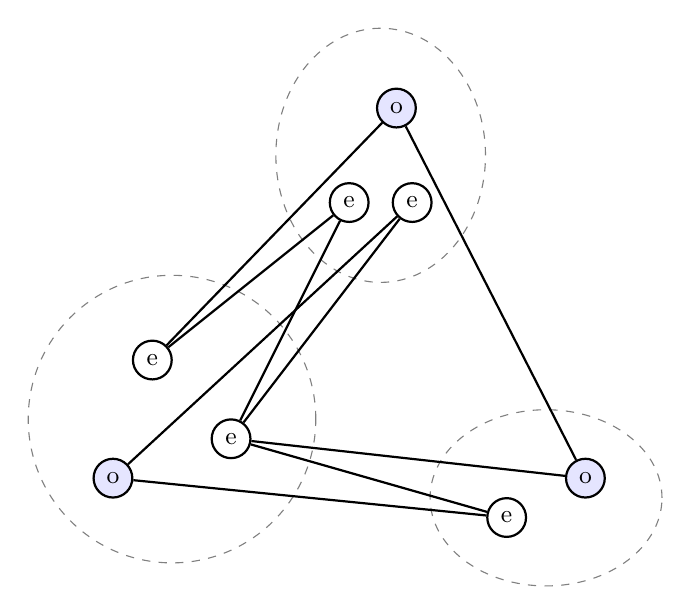
\begin{tikzpicture}[
    vertex/.style={circle, draw=black, thick, minimum size=14pt, inner sep=0pt, font=\small},
    odd/.style={vertex, fill=blue!10},
    even/.style={vertex, fill=white},
    edge/.style={thick, black},
    bag/.style={ellipse, draw=gray, dashed, inner sep=8pt}
]

    % --- Bag A (Top): 1 odd, 2 even ---
    \node[odd]  (Ao)  at (0.6, 5.2)   {o};
    \node[even] (Ae1) at (0, 4) {e};
    \node[even] (Ae2) at (0.8, 4)  {e};
    \node[bag, fit=(Ao) (Ae1) (Ae2)] (BagA) {};

    % --- Bag B (Bottom Left): 1 odd, 3 even ---
    \node[odd]  (Bo)  at (-3, 0.5)   {o};
    \node[even] (Be1) at (-2.5, 2) {e};
    \node[even] (Be2) at (-1.5, 1) {e};
    \node[bag, fit=(Bo) (Be1) (Be2)] (BagB) {};

    % --- Bag C (Bottom Right): 1 odd, 1 even ---
    \node[odd]  (Co)  at (3, 0.5)   {o};
    \node[even] (Ce1) at (2, 0) {e};
    \node[bag, fit=(Co) (Ce1)] (BagC) {};

    % --- Path AB (Length 5: A -> B -> A -> B -> A -> B) ---
    % Path: Ao -- Be1 -- Ae1 -- Be2 -- Ae2 -- Bo
    \draw[edge] (Ao)  -- (Be1);
    \draw[edge] (Be1) -- (Ae1);
    \draw[edge] (Ae1) -- (Be2);
    \draw[edge] (Be2) -- (Ae2);
    \draw[edge] (Ae2) -- (Bo);

    % --- Path BC (Length 3: B -> C -> B -> C) ---
    % Path: Bo -- Ce1 -- Be3 -- Co
    \draw[edge] (Bo)  -- (Ce1);
    \draw[edge] (Ce1) -- (Be2);
    \draw[edge] (Be2) -- (Co);

    % --- Path CA (Length 1: C -> A) ---
    % Path: Co -- Ao
    \draw[edge] (Co) -- (Ao);

\end{tikzpicture}

    \caption{An example of a graph with an oddomorphism to $K_3$. The fibres of the oddomorphism are indicated by the dashed lines.}
    \label{fig:oddo_example}
\end{figure}




\section{The Strong Roberson Conjecture cannot be proved using oddomorphisms}
\label{sec:oddo-doesnt-mean-minor}
In this section we resolve Question \ref{q} in the negative.
In fact, we give two different constructions showing that the existence of an oddomorphism (and thus a weak oddomorphism) from $F$ to $G$ need not imply that $F$ contains $G$ as a minor. The first is a new construction while the second is drawn from the literature. Identifying it as a counterexample requires only a minor observation.

\subsection{First example: Gluing of 5-cycles}
\label{sec:first-counterexample}
The construction of this example requires some preparation before it can be presented.
A key step is to transfer the problem to the more restrictive setting of rooted minors. Then it suffices to find examples of graphs $G$ and $F$ such that $G$ is not a rooted minor of $F$ with some prescribed labels.
\par 
The following lemma is an application of a fairly standard technique in structural graph theory, but we give a proof for completeness.
\begin{lemma}
\label{lemma:rooted-minors}
    Let $F$ and $G$ be connected graphs and let $v_1,\ldots, v_n$ be distinct vertices in $G$ and $w_1,\ldots, w_n$ be distinct vertices in $F$.
    The graphs $F$ and $G$ can be extended to graphs $F_+$ and $G_+$  satisfying the following: $G_+$ is a minor of $F_+$ if and only if there is a partial function $\pi: V(F) \rightharpoonup V(G)$ witnessing the fact that $G$ is a minor of $F$ and additionally satisfying $\pi(w_i) = v_i$ for each $i \in \{1,\ldots, n\}$.
\end{lemma}
\begin{proof}
    Let $D$ be the sum of the degrees of the vertices in $V(F)$. We construct $F_+$ from $F$ by adding $D\cdot 2^i$ degree 1 vertices adjacent to the vertex $w_i$ for each $i$. Similarly we construct $G_+$ from $G$ by adding $D\cdot 2^i$ degree 1 vertices adjacent to $v_i$ for each $i$.
    If $\pi$ witnesses the fact that $G$ is a minor of $F$ and $\pi(w_i) = v_i$ for each $i$, we can extend $\pi$ to a witness of the fact that $G_+$ is a minor of $F_+$ by bijectively mapping the new degree 1 vertices. 
    \par
    For the other direction, let $\pi_+: F_+ \rightharpoonup G_+$ witness the fact that $G_+$ is a minor of $F_+$. 
    For each $i$, the sum of the degrees of the vertices in $\pi_+^{-1}(v_i)$ must be at least $D\cdot 2^i$. 
    We take as an induction hypothesis that $w_j \in \pi_+^{-1}(v_j)$ for each $j>i$. The sum of the degrees of the remaining vertices excluding $w_i$ is $\sum_{0\leq j<i} D \cdot 2^j < D\cdot 2^i$, so it follows that $w_i$ must belong to the fibre $\pi_+^{-1}(v_i)$. Using induction we see that this holds for all $i\in \{1,\ldots, n\}$.
    Additionally, if $\pi_+$ maps a degree 1 vertex that is adjacent to $w_i$ and is outside of $F$ to a vertex inside $V(G)\setminus \{v_i\}$, that vertex must be a degree 1 vertex in $G_+$ that is adjacent to $v_i$. It is easy to see that such vertices can be permuted to define a partial function $\pi_+'$ that is equal to $\pi_+$ everywhere except at those degree 1 vertices and whose restriction to $V(F)$ is onto $V(G)$. This restriction is then the witness $\pi$ of the fact that $G$ is a minor of $F$ which additionally satisfies $\pi(w_i) = v_i$ for each $i$.
\end{proof}

To take advantage of Lemma \ref{lemma:rooted-minors}, we must show that oddomorphisms can be extended to the extensions $F_+$ and $G_+$.
We show the slightly more general fact that they can indeed be extended by gluing a graph to both the domain and codomain.\par 
For graphs $G$ and $H$ with $v$ a vertex in $G$ and $h$ a vertex in $H$ we let $G_v \oplus H_h$ denote the gluing of $G$ and $H$ on the vertices $v$ and $h$. More specifically, $G_v \oplus H_h$ can be constructed by taking the disjoint union of $G$ and $H$, adding the edge $\{v,h\}$ and then contracting it.

\begin{lemma}
\label{lemma:oddo_extension}
    Let $\psi: F \to G$ be an oddomorphism, $v$ be a vertex of $G$, and let $H$ be a graph with a vertex $h$. If there is exactly one $\psi$-odd vertex $u$ in $\psi^{-1}(v)$, then $\psi$ extends to an oddomorphism $\psi_+:F_u \oplus H_h \to G_v \oplus H_h$ by mapping the non-$h$ elements of $H$ to themselves.
\end{lemma}
\begin{proof}
    In the new oddomorphism, all of the new elements added from $H$ in $F_u \oplus H_h$ are labelled odd, and the others keep their labels. 
    The number of odd vertices in a fibre $\psi_+^{-1}(a)$ for $a \in V(G)$ is unaffected by the gluing. Likewise, for $e \in E(G)$, the induced subgraph of $F_u \oplus H_h$ on $\psi_+^{-1}(e)$ is the same graph as the induced subgraph of $F$ on $\psi^{-1}(e)$. The degree condition therefore also holds for these edges.
\par 
    Each fibre $\psi_+^{-1}(a)$ for $a \in V(H) \setminus \{h\}$ contains precisely one element, so the condition that each fibre contains an odd number of odd elements is also satisfied for these vertices. To see that the degree condition is satisfied on the $\psi_+$-preimages of edges $e$ in $H$ we note that the induced subgraph of $F_u \oplus H_h$ on $\psi_+^{-1}(e)$ is just a single edge between the corresponding odd vertices. So it is clear that each odd vertex has degree 1 in this graph while an even vertex has degree 0.
\end{proof}

\begin{figure}[ht]
    \centering
    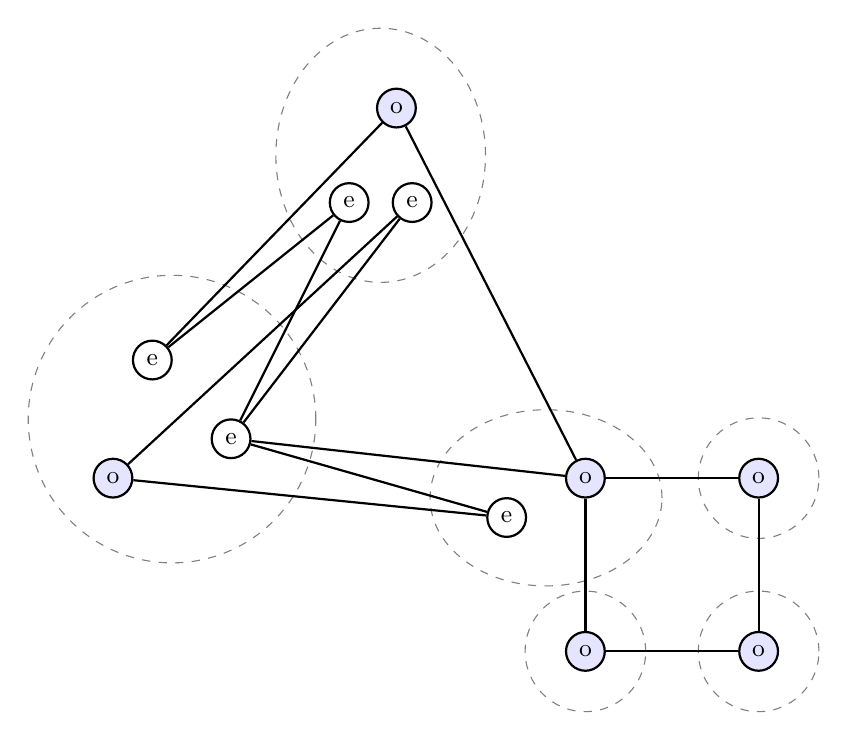
\begin{tikzpicture}[
    vertex/.style={circle, draw=black, thick, minimum size=14pt, inner sep=0pt, font=\small},
    odd/.style={vertex, fill=blue!10},
    even/.style={vertex, fill=white},
    edge/.style={thick, black},
    bag/.style={ellipse, draw=gray, dashed, inner sep=8pt},
]

    % --- Bag A (Top): 1 odd, 2 even ---
    \node[odd]  (Ao)  at (0.6, 5.2)  {o};
    \node[even] (Ae1) at (0, 4)     {e};
    \node[even] (Ae2) at (0.8, 4)   {e};
    \node[bag, fit=(Ao) (Ae1) (Ae2)] (BagA) {};

    % --- Bag B (Bottom Left): 1 odd, 2 even ---
    \node[odd]  (Bo)  at (-3, 0.5)   {o};
    \node[even] (Be1) at (-2.5, 2)  {e};
    \node[even] (Be2) at (-1.5, 1)  {e};
    \node[bag, fit=(Bo) (Be1) (Be2)] (BagB) {};

    % --- Bag C (Bottom Right): 1 odd, 1 even ---
    \node[odd]  (Co)  at (3, 0.5)    {o};
    \node[even] (Ce1) at (2, 0)      {e};
    \node[bag, fit=(Co) (Ce1)] (BagC) {};

    % --- New C4 Cycle glued to Co ---
    % Vertices
    \node[odd] (C4a) at (5.2, 0.5)  {o};
    \node[odd] (C4b) at (5.2, -1.7)   {o};
    \node[odd] (C4c) at (3, -1.7)     {o};
    
    % Dotted bags for the new vertices
    \node[bag, fit=(C4a)] {};
    \node[bag, fit=(C4b)] {};
    \node[bag, fit=(C4c)] {};

    % --- Path AB ---
    \draw[edge] (Ao)  -- (Be1);
    \draw[edge] (Be1) -- (Ae1);
    \draw[edge] (Ae1) -- (Be2);
    \draw[edge] (Be2) -- (Ae2);
    \draw[edge] (Ae2) -- (Bo);

    % --- Path BC ---
    \draw[edge] (Bo)  -- (Ce1);
    \draw[edge] (Ce1) -- (Be2);
    \draw[edge] (Be2) -- (Co);

    % --- Path CA ---
    \draw[edge] (Co) -- (Ao);

    % --- Edges for the C4 Cycle ---
    \draw[edge] (Co)  -- (C4a);
    \draw[edge] (C4a) -- (C4b);
    \draw[edge] (C4b) -- (C4c);
    \draw[edge] (C4c) -- (Co);

\end{tikzpicture}
    \caption{The oddomorphism obtained by gluing $C_4$ to the oddomorphism in Figure \ref{fig:oddo_example}}
    \label{fig:oddo_glued_example}
\end{figure}


We can now deduce the main technical lemma of this section. It shows that when looking for an example answering Question \ref{q} in the negative, we can impose additional constraints on the minor map. Namely, it needs to coincide with the oddomorphism on odd vertices that do not share a fibre with other odd vertices.
\begin{lemma}
\label{lemma:labelled-minors}
    Let $F$ and $G$ be connected graphs, $\psi: F \to G$ be an oddomorphism, $S$ be a set of vertices in $G$ such that the $\psi$-fibres of each element of $S$ contain exactly one $\psi$-odd vertex, and $\rho: S \to V(F)$ be the function that picks out this unique $\psi$-odd vertex.
    Then there exist graphs $F_+,G_+$ that extend $F,G$ and an oddomorphism $\psi_+: F_+\to G_+$ such that $G_+$ is a minor of $F_+$ if and only if there is a partial function $\pi: V(F) \rightharpoonup V(G)$ witnessing the fact that $G$ is a minor of $F$ which satisfies the condition that $\pi(\rho(s)) = s$ for each $s \in S$.
\end{lemma}
\begin{proof} 
    Observe that in the proof of Lemma \ref{lemma:rooted-minors} the graphs $F_+$ and $G_+$ were constructed by gluing star graphs to $F$ and $G$, respectively. It therefore follows from Lemma \ref{lemma:oddo_extension} that an oddomorphism $F \to G$ can be extended to an oddomorphism from $F_+$ to $G_+$, where $F_+$ and $G_+$ are constructed as in Lemma \ref{lemma:rooted-minors} with $S = \{v_1,\ldots, v_n\}$ and $w_i = \rho(v_i)$. The result now follows from Lemma \ref{lemma:rooted-minors}.
\end{proof}

We now construct graphs $A$ and $B$ that will form the foundation of our example.
We define $B$ as the gluing of two cycles of length 5 at a single vertex (see Figure \ref{fig:G}). More specifically, it consists of vertices $\{c, v_1, v_2, v_3, v_4, w_1, w_2, w_3, w_4\}$ where $E(B) = \{ \{v_i, v_{i+1 \mod 5}\} \mid i \in \{0,\ldots, 4\}\} \cup \{ \{w_i, w_{i+1 \mod 5}\} \mid i \in \{0,\ldots, 4\}\}$ where $ v_0 = c = w_0$. 

\begin{figure}[htbp]
    \centering
    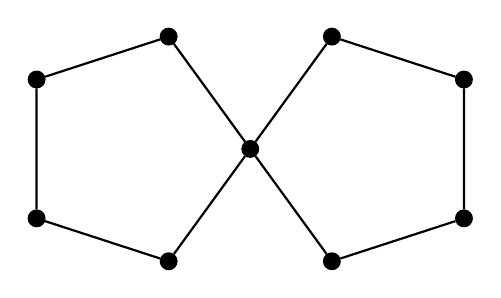
\begin{tikzpicture}[
    % Define the style for the vertices
    vertex/.style={circle, draw, fill=black, inner sep=2pt},
    % Define the thickness of the edges
    thick
]

    % --- Configuration ---
    \def\radius{1.5cm} % Radius of the pentagons

    % --- The Shared Central Vertex ---
    \node[vertex] (center) at (0,0) {};

    % --- Left Cycle (Pentagon 1) ---
    % Geometric center is at (-\radius, 0).
    % We define nodes starting from the shared vertex (at 0 degrees relative to geometric center)
    % and going counter-clockwise: 72, 144, 216, 288.
    \foreach \angle [count=\i] in {72, 144, 216, 288} {
        \node[vertex] (L\i) at ($(-\radius,0) + (\angle:\radius)$) {};
    }
    
    % Draw the edges for the Left Cycle
    \draw (center) -- (L1) -- (L2) -- (L3) -- (L4) -- (center);

    % --- Right Cycle (Pentagon 2) ---
    % Geometric center is at (\radius, 0).
    % The shared vertex is at 180 degrees relative to this geometric center.
    % We place other nodes at: 180+72, 180+144, etc.
    \foreach \angle [count=\i] in {252, 324, 36, 108} {
        \node[vertex] (R\i) at ($(\radius,0) + (\angle:\radius)$) {};
    }

    % Draw the edges for the Right Cycle
    \draw (center) -- (R1) -- (R2) -- (R3) -- (R4) -- (center);

\end{tikzpicture}
    \caption{The graph $B$.}
    \label{fig:G}
\end{figure}
\par 
The graph $A$, along with the oddomorphism $\varphi:A \to B$, is constructed by making each fibre consist of a single odd and a single even vertex, and each bipartite graph between such fibres a path of length 3 starting and ending at the odd vertices (see Figure \ref{fig:F}). More specifically, for a vertex $u \in V(B)$ there are two vertices $(u,o), (u,e) \in V(A)$. If $\{u,t\} \in E(B)$ then $\{(u,o), (t,e)\}, \{(t,e), (u,e)\}, \{(u,e), (t,o)\} \in E(A)$. Then we can define $\varphi: (u,x) \mapsto u$ where $x \in \{o,e\}$.


\begin{figure}[htbp]
    \centering
    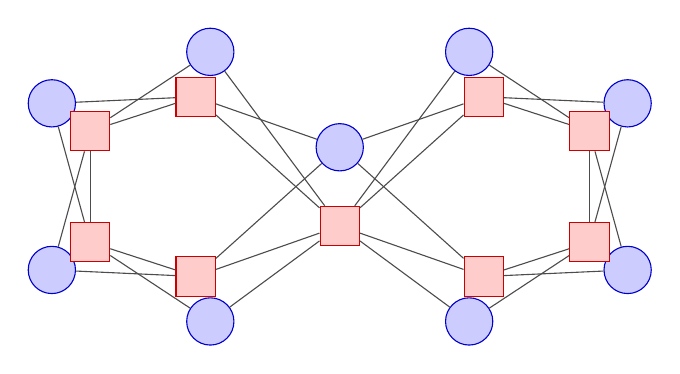
\begin{tikzpicture}[
    % Define styles for the two types of vertices
    v_odd/.style={circle, draw=blue!80!black, fill=blue!20, inner sep=2pt, minimum size=6mm, font=\tiny},
    v_even/.style={rectangle, draw=red!80!black, fill=red!20, inner sep=2.5pt, minimum size=5mm, font=\tiny},
    % Define edge style
    edge/.style={draw=black!70, thin}
]

    % --- Configuration ---
    \def\cycleRadiusOdd{1.8cm}  % Radius for Odd nodes
    \def\cycleRadiusEven{1.2cm} % Radius for Even nodes
    \def\shift{2.2cm}           % Distance of pentagon centers from origin

    % --- Helper Macro for Connections ---
    % Arguments: (u_odd, u_even, v_odd, v_even)
    % Logic: Path u_odd -- v_even -- u_even -- v_odd
    \newcommand{\connectbags}[4]{
        \draw[edge] (#1) -- (#4);
        \draw[edge] (#4) -- (#2);
        \draw[edge] (#2) -- (#3);
    }

    % --- The Central Bag (Shared Vertex) ---
    % We place this at (0,0). To avoid overlap, we stack them vertically.
    \node[v_odd] (C_o) at (0, 0.5) {};
    \node[v_even] (C_e) at (0, -0.5) {};


    % ================= LEFT CYCLE =================
    % Geometric center at (-\shift, 0)
    % We need 4 more bags (indices 1 to 4) to complete the 5-cycle.
    % Angles relative to (-\shift, 0):
    % The Center bag acts as the 0-degree neighbor.
    % We place others at 72, 144, 216, 288.
    
    \foreach \angle [count=\i] in {72, 144, 216, 288} {
        % Calculate coordinates relative to the left center
        \coordinate (origin) at (-\shift,0);
        \node[v_odd]  (L\i_o) at ($(origin) + (\angle:\cycleRadiusOdd)$) {};
        \node[v_even] (L\i_e) at ($(origin) + (\angle:\cycleRadiusEven)$) {};
    }

    % --- Connect Left Cycle ---
    % 1. Center Bag <-> L1
    \connectbags{C_o}{C_e}{L1_o}{L1_e}
    % 2. L1 <-> L2 <-> L3 <-> L4
    \connectbags{L1_o}{L1_e}{L2_o}{L2_e}
    \connectbags{L2_o}{L2_e}{L3_o}{L3_e}
    \connectbags{L3_o}{L3_e}{L4_o}{L4_e}
    % 3. L4 <-> Center Bag
    \connectbags{L4_o}{L4_e}{C_o}{C_e}


    % ================= RIGHT CYCLE =================
    % Geometric center at (\shift, 0)
    % Center bag acts as the 180-degree neighbor.
    % We place others at 180+72, 180+144, etc. -> 252, 324, 36, 108
    
    \foreach \angle [count=\i] in {252, 324, 36, 108} {
        \coordinate (origin) at (\shift,0);
        \node[v_odd]  (R\i_o) at ($(origin) + (\angle:\cycleRadiusOdd)$) {};
        \node[v_even] (R\i_e) at ($(origin) + (\angle:\cycleRadiusEven)$) {};
    }

    % --- Connect Right Cycle ---
    % 1. Center Bag <-> R1
    \connectbags{C_o}{C_e}{R1_o}{R1_e}
    % 2. R1 <-> R2 <-> R3 <-> R4
    \connectbags{R1_o}{R1_e}{R2_o}{R2_e}
    \connectbags{R2_o}{R2_e}{R3_o}{R3_e}
    \connectbags{R3_o}{R3_e}{R4_o}{R4_e}
    % 3. R4 <-> Center Bag
    \connectbags{R4_o}{R4_e}{C_o}{C_e}

\end{tikzpicture}
    \caption{Our graph $A$. The red squares are the even vertices and the blue circles are the odd vertices. The pairs of odd-even vertices that are next to each other in the figure form the fibres of the oddomorphism $\varphi:A \to B$.}
    \label{fig:F}
\end{figure}

The key property of these graphs is the following:
\begin{proposition}
    Let $A$, $B$, and $\varphi$ be defined as in the preceding text. There is no partial function $\pi: V(A) \rightharpoonup V(B)$ which witnesses the fact that $B$ is a minor of $A$ and also coincides with $\varphi$ on the $\varphi$-odd vertices of $A$.
\end{proposition}
\begin{proof}
    This is relatively simple to check by hand. Assume $\pi$ is such a partial function. To derive a contradiction, we examine two cases. For the remainder of this proof, a fibre is always a fibre of $\pi$.\begin{itemize}
        \item Assume $(c, e)$ is mapped to $c$ under $\pi$. Since $\pi^{-1}(c)$ is connected and it contains $(c,o)$ it must include another even vertex. Assume without loss of generality that it contains $(v_1, e)$.  
        Now, $(v_1,o) \in \pi^{-1}(v_1)$ and this fibre must be adjacent to the fibre containing $(v_2,o)$, so $(v_2,e)$ must be contained in either $\pi^{-1}(v_1)$ or $\pi^{-1}(v_2)$.
        In both cases $(v_3,e)$ must be contained in the same fibre as $\pi^{-1}(v_2)$.
        But then $\pi^{-1}(v_4)$ can only consist of $(v_4,o)$ and is therefore not adjacent to $\pi^{-1}(v_3)$, a contradiction.

        \item Assume $(c, e)$ is not mapped to $c$ under $\pi$.
        Now, assume without loss of generality that $\pi((c,e)) = w_i$ for some $i \in \{1,2,3,4\}$. Since $\pi^{-1}(c)$ must be adjacent to both $\pi^{-1}(v_1)$ and $\pi^{-1}(v_4)$ it follows that $(v_1,e)$, $(v_2,e)$, $(v_3,e)$, and $(v_4,e)$ must all be contained in $\pi^{-1}(c) \cup \pi^{-1}(v_1) \cup \pi^{-1}(v_4)$ (since the only valid paths from $(c,o)$ to $(v_1,o)$ and $(v_4,o)$ go through these vertices). But then $\pi^{-1}(v_2)$ and $\pi^{-1}(v_3)$ are not adjacent, a contradiction.
    \end{itemize}

    
\end{proof}


It now follows from Lemma \ref{lemma:labelled-minors} that we can construct an oddomorphism $\varphi_+: A_+ \to B_+$ where $B_+$ is not a minor of $A_+$. We have thus resolved Question \ref{q} by showing:
\begin{theorem}
    There exists a pair of graphs $F$, $G$ such that there is an oddomorphism $F \to G$ but $G$ is not a minor of $F$.
\end{theorem}


This therefore shows that the class of graphs obtained by excluding $G = B_+$ as a minor is not closed under oddomorphisms while still being minor closed.
Additionally, $B$ is planar and $B_+$ is obtained by adding leaves to $B$, so $B_+$ is also planar. It then follows from a celebrated result by Robertson and Seymour \cite{ROBERTSON198692} that this class of graphs that exclude $B_+$ as a minor has bounded treewidth.
Thus the statement that a minor closed class is closed under oddomorphisms fails even for classes of bounded treewidth.
This observation was made by Tim Seppelt (personal communication).



\subsection{Second example: Random lifts of cliques}
The second example follows from work by Drier and Linial on the Hadwiger number of random lifts of complete graphs \cite{Drier2004Minors}. \par 
For a positive integer $l$, an \emph{$l$-lift} of a graph $G$ is a graph with vertex set $V(G) \times [l]$ and an edge set consisting of perfect matchings between $\{u\} \times [l]$ and $\{v\} \times [l]$ for each $\{u,v\} \in E(G)$. We say that $F$ is a \emph{lift} of $G$ if it is an $l$-lift of $G$ for some positive integer $l$.
\par 
The key observation explaining the relevance of this work for our purposes is that odd lifts are examples of oddomorphisms.
\begin{proposition}
    Let $G_l$ be an $l$-lift of a graph $G$ where $l$ is an odd number. Then the projection $V(G) \times [l] \to V(G)$ is an oddomorphism $G_l \to G$.
\end{proposition}
\begin{proof}
    The projection is clearly a homomorphism.
    We let every vertex of $G_l$ be odd. Since $l$ is odd, this means that there is an odd number of odd vertices in each fibre of the projection. The inverse image of an edge in $G$ is, by definition, a perfect matching in $G_l$. Therefore each vertex has degree 1 in that subgraph and thus they all satisfy the degree condition.
\end{proof}

A \emph{random $l$-lift} of a graph $G$ is an $l$-lift of $G$ such that for each $\{u,v\} \in E(G)$ the perfect matching between $\{u\} \times [l]$ and $\{v\} \times [l]$ is chosen uniformly at random.

\begin{lemma}[Lemma 3.8 in \cite{Drier2004Minors}]
\label{lemma:Drier}
    For every $\delta,\varepsilon>0$ there exists $n$ large enough such that for each $2\leq l \leq (\frac14 - \varepsilon) \log n$ the probability that a random $l$-lift of $K_n$ contains $K_n$ as a minor is less than $\delta$.
\end{lemma}

In particular, we can pick $l$ as a constant, for example $l =3$. It then follows from Lemma \ref{lemma:Drier} that for large $n$, almost all of the random $3$-lifts of $K_n$ do not contain $K_n$ as a minor. 
As these lifts have an oddomorphism to $K_n$, this gives an infinite class of examples confirming the negative answer to Question \ref{q}.



\section{The Strong Roberson Conjecture for split-off minors is true}
\label{sec:oddo-means-som}
In the previous section we showed that the existence of an oddomorphism from $F$ to $G$ is not enough to ensure that $F$ contains $G$ as a minor. In this section we show that a slightly weaker relation between $F$ and $G$ holds. Namely, that $F$ contains $G$ as a split-off minor.

\begin{definition}
\label{def:split-off-minors}
    A multigraph $H$ is a \emph{split-off minor} of a multigraph $G$ if $H$ can be obtained from $G$ by applying the operations of taking subgraphs, contracting edges, and splitting off edges (both considered as multigraph operations).
\end{definition}

In particular, if $G$ and $H$ are simple graphs, we say that $G$ contains $H$ as a split-off minor if $H$ can be obtained from $G$ by applying these operations as multigraph operations. Thus the graphs in the intermediate steps can have multiple edges.
\par 
The split-off minor relation is a natural one to consider when studying classes closed under such operations. Indeed, a class of multigraphs is closed under taking split-off minors if and only if it is closed under both minors and immersions. See Proposition \ref{prop:split-off-closure} for further details.

\par 
The split-off minor relation has not been studied previously in the literature. 
Golovach et al. \cite{GOLOVACH2014286} examined a very similar relation which they call the \emph{lift-minor} relation.
Their relation is defined using the same operation. However, they restrict themselves only to simple graphs. Additionally, they consider the operations as simple graph operations, so multiple edges are always merged into single edges when they arise and loops are always deleted.
\par 


The goal of this section is to prove Theorem \ref{thm:oddo-implies-lm}.
We begin by proving it in the case where $F$ is a lift of $G$.

\begin{lemma}
\label{lemma:perfect-matching-lm}
    If $F$ is a lift of a graph $G$ then $G$ is a split-off minor of $F$.
\end{lemma}
\begin{proof}
    Let $\varphi:F\to G$ be the projection and let $T$ be a full spanning forest in $G$, meaning that each component of it is a spanning tree of a component of $G$. 
    An $l$-lift of a forest consists of $l$ isomorphic copies of that forest. We therefore see that there exists a subforest $T_F$ in $F$ such that $\varphi$ restricts to an isomorphism $T_F \to T$.
    \begin{claim}
    \label{claim:tree-paths}
        For each $x,y \in T_F$ that lie on the same tree in $T_F$ and satisfy $\{\varphi(x), \varphi(y)\} \in E(G) \setminus E(T)$ there exists a path $P_{x,y}$ between $x$ and $y$ that is disjoint from $T_F$ except at its endpoints, and additionally the first and last edge of the path both map to $\{\varphi(x), \varphi(y)\}$ under $\varphi$.
    \end{claim}
    \begin{proofofclaim}
        Assume $x$ and $y$ are as stated above. Note that there is a cycle $C$ in $G$ consisting only of the edge $\{\varphi(x), \varphi(y)\}$ and edges from $T$. The induced subgraph of $F$ on the vertices of $\varphi^{-1}(C)$ is a lift of $C$, so every vertex in it has degree 2 and it is therefore a disjoint union of cycles. Note that the path between $x$ and $y$ which lies in the tree $T_F$ is contained in this subgraph and thus $x$ and $y$ lie on the same cycle $C'$ within $\varphi^{-1}(C)$. Taking the other path between $x$ and $y$ on that cycle gives a path between $x$ and $y$ that is disjoint from $T_F$ except at its endpoints. 
        The first and last edges of this path do not map to $T$ under $\varphi$, since if that were the case $x$ or $y$ would have degree larger than 1 within the preimage of the edge mapped to, contradicting the fact that this preimage is a perfect matching. Thus these first and last edges must map to the only edge of $C$ not in $T$, which is $\{\varphi(x), \varphi(y)\}$.
    \end{proofofclaim}

    We now form a graph $F'$ from $F$ by contracting every edge $e$ both of whose endpoints lie outside of $T_F$. Note that $F'$ is not necessarily a simple graph.
    We prove that $G$ immerses into $F'$. For the branch vertex function we use the inverse of $\varphi$ on $T_F$, that is $(\restr{\varphi}{T_F})^{-1}$. For $e \in E(T)$ we define $P_e$ as the path consisting only of the corresponding edge in $T_F$. For edges $e$ outside of $T$, we define $P_e$ as the path in $F'$ corresponding to the path obtained from Claim \ref{claim:tree-paths}. 
    All that remains is to show that two such paths are edge disjoint. Let $\{x,y\}, \{x',y'\} \in E(G)\setminus E(T)$ be two distinct edges corresponding to such paths. These paths have length 2, since only the first and last edges of a path obtained from Claim \ref{claim:tree-paths} have an endpoint in $T_F$, so the other edges were contracted in the formation of $F'$. The two remaining edges which $P_{\{x,y\}}$ consists of map to $\{\varphi(x), \varphi(y)\}$ and the two edges of $P_{\{x',y'\}}$ map to $\{\varphi(x'), \varphi(y')\}$ under $\varphi$. 
    Since $G$ is simple we can assume without loss of generality that $y' \notin \{x,y\}$. 
    Then, since $\varphi$ is a bijection on $V(T_F)$ we have that $\varphi(y') \notin \{\varphi(x), \varphi(y)\}$ and thus
    \begin{align*}
        \{\varphi(x), \varphi(y)\} \neq \{\varphi(x'), \varphi(y')\}.
    \end{align*}
    It then follows that the set of edges forming $P_{\{x,y\}}$ must be disjoint from the set of edges forming $P_{\{x',y'\}}$. This completes the proof.
\end{proof}

We can now prove the full theorem.

\begin{proof}[Proof of Theorem \ref{thm:oddo-implies-lm}]
    Assume $\varphi$ is an oddomorphism $F \to G$. 
    We can assume that $G$ is connected since the oddomorphism induces an oddomorphism to each component. Additionally, the result is trivial if $G$ is the single vertex graph, so we assume $G$ has at least one edge and thus has no isolated vertices.
    \par 
    For $e \in E(G)$ let $F_e$ be the induced subgraph of $F$ on the vertices in $\varphi^{-1}(e)$. Then $\{E(F_e) \mid e \in E(G)\}$ is a partition of $E(F)$.
    Let $A_e$ be a maximal set of edge-disjoint circuits in $F_e$. We begin by deleting all edges forming a circuit in $A_e$ to form the graph $F_e'$. We then repeatedly split off a maximal length path of length $>1$ within $F_e'$, one at a time, until no such paths are left. Let $F_e''$ be the resulting graph and let $X_e \coloneqq E(F_e'')$.
    We define $F''$ as the graph obtained from the graph $(V(F), \bigcup_{e \in E(G)} X_e)$ by deleting all isolated vertices. Clearly $F''$ is an immersion of $F$ and $\{X_e \mid e \in E(G)\}$ is a partition of the edges of $F''$.
    % For $e \in E(G)$ let $F_e$ be the induced subgraph of $F$ on the vertices in $\varphi^{-1}(e)$.
    % Let $A_e$ be a maximal set of edge-disjoint circuits in $F_e$. We begin by deleting all edges forming a circuit in $A_e$, for each $e$.
    % We then repeatedly split off a maximal length path of length $>1$ within what remains of $F_e$, one at a time, until no such paths are left. Let $F''$ be the resulting multigraph when these operations have been applied for every $e \in E(G)$ and we have deleted all isolated vertices.
    An example of this construction of $F''$ is illustrated in Figure \ref{fig:oddo-split-minor-example}.
    % We have a partition $\{ X_e \mid e \in E(G) \}$ of the edges of $F''$ defined by the following: For $f \in E(F'')$ we have $f \in X_e$ if and only if $f$ is in $F_e$ or it was formed from a path within $F_e$ which was split off.
    \begin{claim}
        The vertices of $F''$ are exactly the $\varphi$-odd vertices of $F$ and every vertex $v \in V(F'')$ is incident to exactly one edge in $X_e$ for each $e \in E(G)$ with $v \in V(F_e) = \varphi^{-1}(e)$.
    \end{claim}
    \begin{proofofclaim}
        First, note that the parity of the degree of a vertex in $F_e'$ is equal to the parity of its degree in $F_e$, since each vertex in a circuit has even degree.
        Similarly, the parity of the degree of a vertex in $F_e''$ is equal to the parity of its degree in $F_e'$, since when a pair of edges is split off from a vertex the degree of the vertex decreases by 2 and the degrees of all other vertices remain constant.
        Thus, an odd vertex in $F$ has odd degree in $F_e''$ and is therefore not isolated in $(V(F), \bigcup_{e \in E(G)} X_e)$ so it belongs to $V(F'')$.
        However, an even vertex in $F$ has even degree in $F_e''$. Additionally, if its degree is greater than 1, it lies on a path of length $>1$ in $F_e''$, a contradiction. Thus its degree in $F_e''$ must be 0 for each $e$, so it is isolated in $(V(F), \bigcup_{e \in E(G)} X_e)$ and thus not in $V(F'')$.
        \par 
        By the same argument we see that the degree of an odd vertex in $F_e''$ is not greater than 1, so it must be exactly 1. Therefore, each vertex of $F''$ is incident to exactly one edge in $X_e$ if $v \in \varphi^{-1}(e)$.
    \end{proofofclaim}
    % \begin{claim}
    %     For every $x \in V(F'')$ and every $\{\varphi(x), y\} \in E(G)$ we have that $x$ is incident with exactly one edge in $X_{\{\varphi(x), y\}}$.
    % \end{claim}
    % \begin{proofofclaim}
    %     If $x$ is incident with more than one edge within $X_e$ then there is a path of length $>1$ within $X_e$ (where $e = \{\varphi(x), y\}$). This is a contradiction since all such paths were split off. Nor can it be the case that $x$ has degree 0 within $X_e$ since, as mentioned above, the degree within a part $X_e$ is always reduced by an even amount and $x$ is odd. Thus $x$ has degree $1$ within $X_e$.
    % \end{proofofclaim}
    For $x \in V(G)$, let $H_x$ denote the induced subgraph of $F''$ on the vertices of $\varphi^{-1}(x) \cap V(F'')$.
    \begin{claim}
    \label{claim:odd-even-components}
        A connected component of odd/even size in $H_x$ has an odd/even number of edges connecting it to $H_y$ for any $\{x,y\} \in E(G)$.
    \end{claim}
    \begin{proofofclaim}
        Let $C\subseteq H_x$ be such a component and let $\{x,y \} \in E(G)$. Note that the edges between $H_x$ and $H_y$ are all contained in $X_{\{x,y\}}$ and every edge in $X_{\{x,y\}}$ either connects $H_x$ to $H_y$ or is entirely contained in $H_x$ or $H_y$. 
        Since each vertex in $C$ is incident with exactly one edge in $X_{\{x,y\}}$ and each such edge that is entirely contained in $C$ is incident with two vertices in $C$ (there are no loops) it follows that the parity of the number of edges in $X_{\{x,y\}}$ incident with exactly one vertex of $C$ is the same as the parity of the number of vertices in $C$. This completes the proof of the claim.
    \end{proofofclaim}

    We now let $F_0 \coloneqq F$ and form the graph $F_1$ by contracting all edges in $F''$ that lie within a single fibre of $\varphi$.
    It follows from the preceding claims that $\varphi$ gives rise to a homomorphism $\varphi_1: F_1 \to G$ which is an oddomorphism.
    Indeed, the odd vertices are the components of odd size and the even vertices are the components of even size. Since all vertices of $F''$ are odd, the total number of vertices in a fibre of $F''$ is odd. Thus there is an odd number of odd vertices in each fibre of $\varphi_1$. The degree condition follows directly from Claim \ref{claim:odd-even-components}. 
    \par 

    \begin{figure}[htbp]
        \centering
        \begin{minipage}{0.48\textwidth}
    \centering

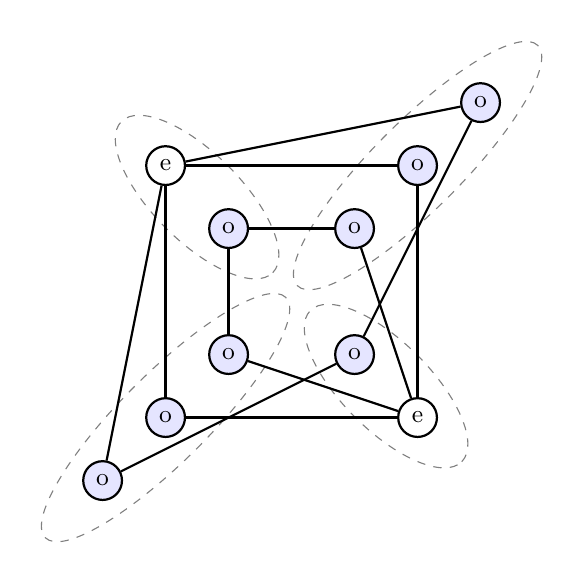
\begin{tikzpicture}[
    vertex/.style={circle, draw=black, thick, minimum size=14pt, inner sep=0pt, font=\small},
    odd/.style={vertex, fill=blue!10},
    even/.style={vertex, fill=white},
    edge/.style={thick, black},
    bag/.style={ellipse, draw=gray, dashed, inner sep=6pt},
    scale=0.8
]

    % --- Bag A (Top left): 
    \node[odd]  (Ao)  at (-1, 1)   {o};
    \node[even] (Ae1) at (-2, 2) {e};
    \node[bag, rotate fit=-45, fit=(Ao) (Ae1)] (BagA) {};

    % --- Bag B (Top right Left):
    \node[odd]  (Bo)  at (1, 1)   {o};
    \node[odd] (Be1) at (2, 2) {o};
    \node[odd] (Be2) at (3, 3) {o};
    \node[bag, rotate fit=45, fit=(Bo) (Be1) (Be2)] (BagB) {};

    % --- Bag C (Bottom Right):
    \node[odd]  (Co)  at (1, -1)   {o};
    \node[even] (Ce1) at (2, -2) {e};
    \node[bag, rotate fit=-45, fit=(Co) (Ce1)] (BagC) {};

    % --- Bag D (Bottom Left)
    \node[odd]  (Do)  at (-1, -1)   {o};
    \node[odd] (De1) at (-2, -2) {o};
    \node[odd] (De2) at (-3, -3) {o};
    \node[bag, rotate fit=45, fit=(Do) (De1) (De2)] (BagD) {};

    \draw[edge] (Ao) -- (Bo);
    \draw[edge] (Ae1) -- (Be1);
    \draw[edge] (Ae1) -- (Be2);
    
    \draw[edge] (Bo) -- (Ce1);
    \draw[edge] (Be1) -- (Ce1);
    \draw[edge] (Be2) -- (Co);

    \draw[edge] (Co) -- (De2);
    \draw[edge] (Ce1) -- (De1);
    \draw[edge] (Ce1) -- (Do);

    \draw[edge] (Ao) -- (Do);
    \draw[edge] (Ae1) -- (De1);
    \draw[edge] (Ae1) -- (De2);
      

\end{tikzpicture}
\end{minipage}\hfill
\begin{minipage}{0.48\textwidth}
    \centering

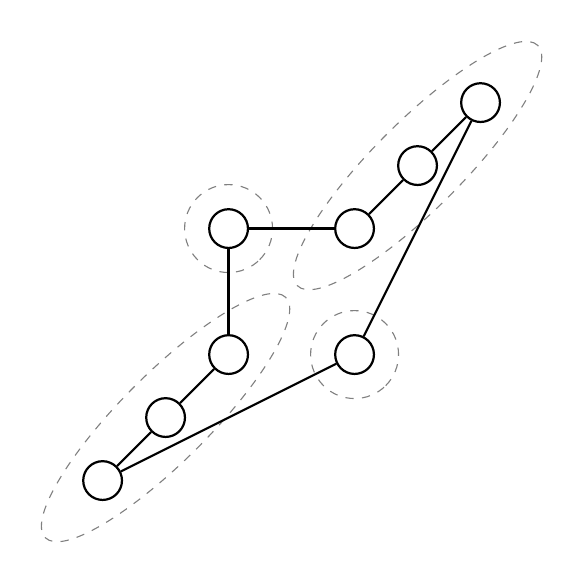
\begin{tikzpicture}[
    vertex/.style={circle, draw=black, thick, minimum size=14pt, inner sep=0pt, font=\small},
    odd/.style={vertex, fill=blue!10},
    even/.style={vertex, fill=white},
    edge/.style={thick, black},
    bag/.style={ellipse, draw=gray, dashed, inner sep=6pt},
    scale=0.8
]

    % --- Bag A (Top left): 
    \node[even] (Ao)  at (-1, 1) {};
    \node[bag, rotate fit=-45, fit=(Ao)] (BagA) {};

    % --- Bag B (Top right Left):
    \node[even]  (Bo)  at (1, 1) {};
    \node[even] (Be1) at (2, 2) {};
    \node[even] (Be2) at (3, 3) {};
    \node[bag, rotate fit=45, fit=(Bo) (Be1) (Be2)] (BagB) {};

    % --- Bag C (Bottom Right):
    \node[even]  (Co)  at (1, -1)   {};
    \node[bag, rotate fit=-45, fit=(Co)] (BagC) {};

    % --- Bag D (Bottom Left)
    \node[even]  (Do)  at (-1, -1)   {};
    \node[even] (De1) at (-2, -2) {};
    \node[even] (De2) at (-3, -3) {};
    \node[bag, rotate fit=45, fit=(Do) (De1) (De2)] (BagD) {};

    \draw[edge] (Ao) -- (Bo);
    \draw[edge] (Be2) -- (Be1);
    
    \draw[edge] (Bo) -- (Be1);
    \draw[edge] (Be2) -- (Co);

    \draw[edge] (Co) -- (De2);
    \draw[edge] (Do) -- (De1);

    \draw[edge] (Ao) -- (Do);
    \draw[edge] (De2) -- (De1);
      

\end{tikzpicture}
\end{minipage}
        \caption{A graph $F$ (left) with an oddomorphism to $C_4$. On the right is the corresponding $F''$. In this case $F_1 = C_4$ and the process would halt after just one iteration.}
        \label{fig:oddo-split-minor-example}
    \end{figure}
    
    We now repeat this process until we get $F_{n+1} = F_n$. Then, for each $e \in E(G)$, there is no circuit within $\varphi_n^{-1}(e)$ and every path within this graph is of length 1. This implies that $\varphi_n^{-1}(e)$ is a matching between the corresponding fibres.
    To see that this matching is perfect, we note that no vertex can have degree 0 within $\varphi_n^{-1}(e)$. A vertex with degree 0 within $\varphi_n^{-1}(e)$ must be even, which implies it has degree 0 in the whole graph since no vertex has degree 2 within any $\varphi_n^{-1}(e')$. This means that the vertex is isolated in $F_n$ and then would have been deleted when forming $F_{n+1}$, a contradiction.
    Thus $F_n$ is a lift of $G$ and it follows from Lemma \ref{lemma:perfect-matching-lm} that $G$ is a split-off minor of $F_n$. Since $F_n$ is a split-off minor of $F$, this completes the proof.
\end{proof}


The following corollary follows from Theorem \ref{thm:oddo-implies-lm} and the fact that a subgraph of a graph $F$ is a split-off minor of $F$.
\begin{corollary}
    \label{cor:wo-implies-som}
    If a graph $F$ has a weak oddomorphism to a graph $G$ then $G$ is a split-off minor of $F$.
    Therefore, a class of graphs that is closed under taking split-off minors is closed under weak oddomorphisms.
\end{corollary}




\section{Split-off minors}
The goal of this section is to establish some facts about the split-off minor relation. 
\par 
We begin by observing that it forms a \emph{well-quasi-ordering}.
One of the most celebrated results in structural graph theory is the result of Robertson and Seymour that the graph minor relation is a well-quasi-ordering on the set of all finite graphs \cite{ROBERTSON2004325}. A well-quasi-ordering is a quasi-order (also known as preorder) that has neither infinite descending chains nor infinite antichains.
In turn, this means that for every class $\C$ of graphs that is closed under taking minors there exists a finite set of graphs $S$ such that $\C$ is the class of graphs that exclude the graphs in $S$ as minors.
The split-off minor relation inherits this property from the minor relation.
\begin{proposition}
\label{prop:split-off-is-wqo}
    The split-off minor relation is a well-quasi-ordering on the set of finite graphs.
\end{proposition}
\begin{proof}
    Since the number of edges or vertices is always reduced when any of the operations are applied, it follows that there are no infinite descending chains. Since a minor is a split-off minor and there are no infinite antichains in the minor relation, it follows that there are no infinite antichains in the split-off minor relation. 
\end{proof}
Note that Robertson and Seymour also proved that the immersion relation is a well-quasi-ordering \cite{ROBERTSON2010181}. We could therefore also have said that the split-off minor relation inherits the well-quasi-ordering property from the immersion relation.
\par
The graph minor and immersion relations have both \emph{constructive} and \emph{structural} definitions. The former is the definition that states that $G$ is a minor/immersion of $F$ if it can be constructed from $F$ by applying a sequence of operations. The latter is the static definition, which is based on whether the structure of the minor/immersion can be exhibited within the larger graph in some way.
\par 
Given this distinction, the definition given here for split-off minors is constructive.
This evokes the question of whether there is also a structural definition for split-off minors. 
It proved difficult to find such a characterisation that is simple, so we settle for one that is quite involved but nevertheless insightful.
Here, we use $\uplus$ to denote the additive union of two multisets and $\setminus$ to denote their subtraction.
\begin{theorem}
    The following are equivalent:
    \begin{enumerate}[(i)]
        \item $G$ is a split-off minor of $F$.
        \item There exists a forest $T$ on $V(F)$, a linear ordering $\prec$ on the edges of $T$, a set of paths $\{P_t \mid t \in E(T)\}$, an injective function $\pi$ from $V(G)$ to the components of $T = (V(F), E(T))$, and a set of paths $\{P_e \mid e \in E(G)\}$ such that \begin{itemize}
            \item For $t \in E(T)$, $P_t$ is a path between the endpoints of $t$ consisting of edges from $(E(F) \setminus \biguplus_{t'\prec t} P_{t'}) \uplus \{t' \mid t'\prec t\}$.
            
            \item $P_{\{u,v\}}$ for $\{u,v\} \in E(G)$ is a path between a vertex in $\pi(u)$ and a vertex in $\pi(v)$, consisting of edges from $(E(F) \setminus \biguplus_{t\in E(T)} P_{t}) \uplus E(T)$.
            \item For any distinct $e,e' \in E(G)$, we have $E(P_e) \cap E(P_{e'}) \subseteq E(T)$.
        \end{itemize}
    \end{enumerate}
\end{theorem}
\begin{proof}\ 
    \begin{itemize}
        \item[(ii)$\Rightarrow$(i)]
            We iterate through the edges $t \in E(T)$ in the order of $\prec$ and first split off the path $P_t$ and then contract the resulting edge $t$. Note that for $t'\prec t$, the edge $t'$ has already been contracted, so, to be precise, we do not split off $P_t$ but the path obtained from $P_t$ by contracting all of the edges $\{t' \mid t'\prec t\}$. Let $F'$ be the resulting graph.
            \par 
            The vertices of $F'$ correspond to the connected components of $T$. Its edges correspond to the edges in $E(F) \setminus \biguplus_{t\in E(T)} P_t$ between the corresponding components of $T$.
            We therefore see that $\pi$ and the paths obtained by contracting all edges in $T$ from $\{P_e \mid e \in E(G)\}$ define an immersion of $G$ into $F'$.
            This shows that $G$ is a split-off minor of $F$.

        \item[(i)$\Rightarrow$(ii)] 
        We define the required objects inductively. 
        First note that if $G = F$, then we can define $T = (V(F), \varnothing)$, $\pi = \id_{V(F)}$, and for $e \in E(G) = E(F)$ we let $P_e$ be the path consisting only of $e$. It is easy to see that all of the conditions are satisfied.\par 
        For the inductive case, let $G'$ be a graph that is a split-off minor of $F$ such that $G$ can be obtained from $G'$ by applying exactly one of the allowed operations. 
        By the induction hypothesis we assume that there exist $T_{G'}$, $\prec_{G'}$, $\{P_t \mid t \in E(T_{G'})\}$, $\pi_{G'}$, and $\{P_e \mid e \in E(G')\}$ satisfying the conditions. 
        We show how the corresponding objects $T_{G}$, $\prec_G$, $\{P_t \mid t \in E(T_{G})\}$, and $\pi_{G}$ are constructed in the four different cases.
        \begin{itemize}
            \item $G$ is obtained from $G'$ by deleting an edge. 
            The only change needed is to delete the path $P_e$ corresponding to the deleted edge $e \in E(G')$.
            \item $G$ is obtained from $G'$ by deleting an isolated vertex. In this case we only have to remove the isolated vertex from the domain of $\pi_{G'}$.

            \item $G$ is obtained from $G'$ by splitting off the edges $\{v,u\}, \{u,w\} \in E(G')$. In this case we remove the paths $P_{\{v,u\}}$ and $P_{\{u,w\}}$ and add $P_{\{v,w\}}$, which is the composition of $P_{\{v,u\}}$, a path within the component of $\pi(u)$ in $T_G$, and $P_{\{u,w\}}$.

            \item $G$ is obtained from $G'$ by contracting an edge $e' \in E(G')$. The set $\{P_e \mid e \in E(G)\}$ is inherited from $G'$ by omitting $P_{e'}$. Let $u,v \in V(F)$ be the endpoints of the path $P_{e'}$. We add a new edge $t$ between $u$ and $v$ to $T_{G'}$ to form $T_G$ and put $t$ at the end of the order $\prec_{G'}$ to form the order $\prec_G$. We then define $P_t$ as the path $P_{e'}$.
            The function $\pi_G$ is equal to $\pi_{G'}$ at all vertices except at the newly merged one. It maps that vertex to the component of $T_{G}$ obtained by joining the components of $T_{G'}$ that contain $u$ and $v$.
        \end{itemize}
         It is easy to check that the constructions $T_{G}$, $\prec_G$, $\{P_t \mid t \in E(T_{G})\}$, and $\pi_{G}$ satisfy the conditions in all of the cases.
    \end{itemize}
\end{proof}
The reason for the necessity of the linear order $\prec$ in the above characterisation is that the order in which the splitting-off and the contraction operations are applied matters. When a splitting-off operation is applied to create an edge that is then contracted, the contraction cannot be applied before the splitting off. Likewise, if a path that is to be split off takes advantage of the fact that two vertices have been merged, the splitting off cannot happen before the contraction (without removing the edge that was contracted to merge the two vertices). It therefore seems necessary to retain some dependency order in the structural definition of split-off minors.

As mentioned previously, the split-off minor relation is very similar to the lift-minor relation studied by Golovach et al. \cite{GOLOVACH2014286}, the only difference being that the multiplicity of edges is always immediately reduced to 1 when forming a lift-minor. It is easy to see that if a graph $G$ is a lift-minor of a graph $F$, then $G$ is a split-off minor of $F$. However, it is not immediately clear whether the two relations are equivalent.
When taking graph minors, whether multiple edges are deleted immediately does not matter, provided that both the initial and final graphs are simple.
An analogous statement holds for immersions, but its proof is not quite immediate.
Since the author was unable to locate a reference for this fact in the literature, a proof is included here.
\begin{proposition}
    Let $G,F$ be simple graphs such that $G$ immerses into $F$. Then $G$ can be obtained from $F$ using the operations of splitting off edges and taking a subgraph in such a way that at every intermediate step the graph is simple.
\end{proposition}
\begin{proof}
    Let $\imm$ denote the immersion relation and let $\immsimp$ denote the relation corresponding to the existence of an immersion where all intermediate graphs are simple.
    Let $(\pi, \{P_e \mid e \in E(G)\})$ be the immersion of $G$ into $F$. 
    We show that we can find a simple graph $F'$ with fewer edges than $F$ such that $G \imm F' \immsimp F$. The result then follows from an induction on the number of edges in $F$.
    To find $F'$ we examine a few cases:
    \begin{itemize}
        \item $F$ contains an edge that does not appear in any $P_e$. We can then let $F'$ be the subgraph of $F$ obtained by deleting that edge. It is clear that $G \imm F' \immsimp F$ and $F'$ has fewer edges than $F$.

        \item $F$ only has edges that appear in some $P_e$ and additionally there exist vertices $v,u,w$ that lie on a path $P_e$ in this order such that $\{v,u\}, \{u,w\} \in E(F)$ but $\{v,w\} \notin E(F)$.
        We then split off the edges $\{v,u\}$ and $\{u,w\}$ to form the graph $F'\immsimp F$. We now show that $G$ immerses into $F'$. To see this, let $P_{e'}$ be the path containing $\{v,u\}$ and let $P_{e''}$ be the path containing $\{u,w\}$. To define the immersion, we leave $\pi$ unchanged along with all $P_f$ for $f \notin \{e,e', e''\}$. The path $P_e$ now takes the new shortcut $\{v,w\}$, the path $P_{e'}$ (if $e' \neq e$) is routed through the old route of $P_e$ between $v$ and $u$, and the path $P_{e''}$ (if $e'' \neq e$) is routed through the old route of $P_e$ between $u$ and $w$.

        \item Neither of the above cases holds. We then have that for each path $P_e$, $F$ contains the complete graph on the vertices of $P_e$. But then $G$ is a subgraph of $F$. Namely, it follows that for each $\{v,u\} \in E(G)$ we have $\{\pi(v), \pi(u)\} \in E(F)$, so $G \imm G \immsimp F$ and we are done.
    \end{itemize}
\end{proof}

In light of these two facts, it is slightly surprising that when the operations of edge-contraction and splitting off are allowed in conjunction, we can no longer require the intermediate steps to be simple and thus the split-off minor relation is not equal to the lift-minor relation.

\begin{proposition}
    There exist simple graphs $F$ and $G$ such that $G$ is a split-off minor of $F$ but $G$ is not a lift-minor of $F$.
\end{proposition}
\begin{proof}[Proof sketch.]
    A result similar to Lemma \ref{lemma:rooted-minors} can be proved for lift-minors and split-off minors. Thus it suffices to find examples of labelled simple graphs $A$ and $B$ such that $B$ is a split-off minor but not a lift-minor of $A$.
    \begin{figure}[htbp]
        \centering
        % First Graph (Top image)
\begin{minipage}{0.48\textwidth}
    \centering
    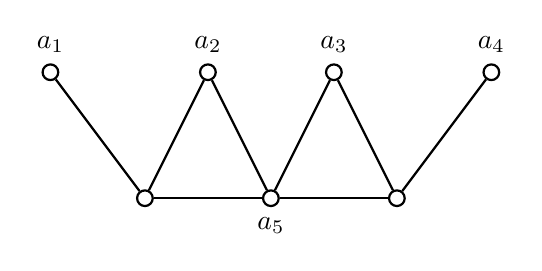
\begin{tikzpicture}[scale=0.8, thick]
        % Define nodes
        \node[circle, draw, inner sep=2pt, label=above:{$a_1$}] (a1) at (0, 2) {};
        \node[circle, draw, inner sep=2pt]                      (u1) at (1.5, 0) {};
        \node[circle, draw, inner sep=2pt, label=above:{$a_2$}] (a2) at (2.5, 2) {};
        \node[circle, draw, inner sep=2pt, label=below:{$a_5$}] (a5) at (3.5, 0) {};
        \node[circle, draw, inner sep=2pt, label=above:{$a_3$}] (a3) at (4.5, 2) {};
        \node[circle, draw, inner sep=2pt]                      (u2) at (5.5, 0) {};
        \node[circle, draw, inner sep=2pt, label=above:{$a_4$}] (a4) at (7, 2) {};

        % Draw edges
        \draw (a1) -- (u1);
        \draw (u1) -- (a2);
        \draw (u1) -- (a5);
        \draw (a2) -- (a5);
        \draw (a5) -- (a3);
        \draw (a5) -- (u2);
        \draw (a3) -- (u2);
        \draw (u2) -- (a4);
    \end{tikzpicture}
\end{minipage}\hfill
% Second Graph (Bottom image)
\begin{minipage}{0.48\textwidth}
    \centering
    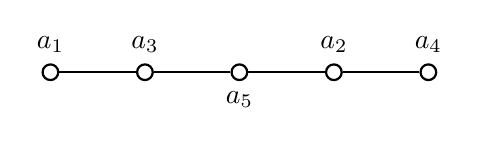
\begin{tikzpicture}[scale=0.8, thick]
        % Define nodes
        \node[circle, draw, inner sep=2pt, label=above:{$a_1$}] (a1) at (0, 0) {};
        \node[circle, draw, inner sep=2pt, label=above:{$a_3$}] (a3) at (1.5, 0) {};
        \node[circle, draw, inner sep=2pt, label=below:{$a_5$}] (a5) at (3, 0) {};
        \node[circle, draw, inner sep=2pt, label=above:{$a_2$}] (a2) at (4.5, 0) {};
        \node[circle, draw, inner sep=2pt, label=above:{$a_4$}] (a4) at (6, 0) {};

        % Draw edges
        \draw (a1) -- (a3);
        \draw (a3) -- (a5);
        \draw (a5) -- (a2);
        \draw (a2) -- (a4);
    \end{tikzpicture}
\end{minipage}

        \caption{The graph $A$ (left) and $B$ (right).}
        \label{fig:lift-minor-counterexample}
    \end{figure}
    
    
    Define $A$ and $B$ and the vertices $\{a_1,\ldots, a_5\}$ as in Figure \ref{fig:lift-minor-counterexample}.
    To obtain $B$ as a split-off minor of $A$ we contract the two edges from $a_5$ to the unlabelled vertices and then split off the paths of length two from $a_1$ to $a_3$, and from $a_2$ to $a_4$.
    \par 
    To see that $B$ is not a lift-minor of $A$ we use brute-force case analysis. This can be checked more easily by a computer program, but we include a check by hand here for completeness.\par 
    We show that if any edge is deleted, contracted, or a pair of edges is split off in $A$ without creating multiple edges, a graph is obtained that does not contain $B$ as a split-off minor.
    A key observation we will use repeatedly is that if a vertex $w$ lies on a path $P$ between $u$ and $v$, it will stay on that path unless the two edges of $P$ that are incident to $w$ are split off.

    \begin{figure}[htbp]
        \centering
        % Define some styles for cleaner code
\tikzset{
    vertex/.style={
        circle,
        draw,
        minimum size=4pt, % Adjust node size
        inner sep=0pt
    },
    label_node/.style={
        draw=none,
        inner sep=1pt,
        anchor=center,
        font=\small % Adjust font size if needed
    },
    c_label/.style={
        label_node,
        above,
        yshift=0.05cm % Shift "c_i" labels slightly further up
    }
}

% Top Graph
\begin{tikzpicture}[scale=1.5]
    % Node definitions based on a grid pattern for spacing
    \node[vertex] (c1) at (0, 1.5) [label={[yshift=0.05cm]above:$a_1$}] {};
    \node[vertex] (v1) at (1, 0) {};
    \node[vertex] (c2) at (2, 1.5) [label={[yshift=0.05cm]above:$a_2$}] {};
    \node[vertex] (c5) at (3, 0) [label={[yshift=-0.05cm]below:$a_5$}] {}; % Label "c_5" further down
    \node[vertex] (c3) at (4, 1.5) [label={[yshift=0.05cm]above:$a_3$}] {};
    \node[vertex] (v2) at (5, 0) {};
    \node[vertex] (c4) at (6, 1.5) [label={[yshift=0.05cm]above:$a_4$}] {};

    % Draw the edges
    \draw (c1) -- (v1);
    \draw (v1) -- (c2);
    \draw (v1) -- (c5);
    \draw (c2) -- (c5);
    \draw (c5) -- (c3);
    \draw (c5) -- (v2);
    \draw (c3) -- (v2);
    \draw (v2) -- (c4);

    % Finer label node placement for edge labels, using coordinate calculations for precision
    \node[label_node] at ($(c1)!0.5!(v1) + (0.05, 0.15)$) {$x$};
    \node[label_node] at ($(v1)!0.5!(c2) + (-0.05, 0.15)$) {$y$};
    \node[label_node] at ($(v1)!0.5!(c5) + (0, -0.15)$) {$r$};
    \node[label_node] at ($(c2)!0.5!(c5) + (0.05, 0.15)$) {$z$};
    \node[label_node] at ($(c5)!0.5!(c3) + (-0.05, 0.15)$) {$z'$};
    \node[label_node] at ($(c5)!0.5!(v2) + (0, -0.15)$) {$r'$};
\end{tikzpicture}

        \caption{}
        \label{fig:lift-minor-counterexample-with-labels}
    \end{figure}
    For ease of reference, we label the edges as in Figure \ref{fig:lift-minor-counterexample-with-labels}.
    \begin{itemize}
        \item Edge deletion. Up to symmetry, we need to explore four cases.
        \begin{itemize}
            \item Delete $x$. Then $a_1$ is isolated, which is a property preserved by split-off minors, so the resulting graph cannot contain $B$ as a split-off minor.
            \item Delete $y$. Then $a_2$ has degree 1 and its degree cannot be increased by merging it with other vertices without merging it with $a_5$, which is forbidden. This graph therefore cannot contain $B$ as a split-off minor.
            
            \item Delete $r$. Then every path between $a_1$ and $a_3$ goes through $a_2$. Again, $a_2$ cannot be merged with other vertices to increase its degree. Thus $a_2$ will be isolated after splitting off the path around it.

           \item Delete $z$. The argument is similar to the previous cases.
        \end{itemize}
        \item Splitting off edges. We only need to explore cases that do not create multiple edges.
        \begin{itemize}
            \item Split off $(x,y)$. As before, $a_2$ lies on the only path between $a_1$ and $a_3$ and it cannot be merged to increase its degree.
            \item Split off $(x,r)$. This creates a leaf at the other endpoint of $y$. This leaf can clearly not be used to find the split-off minor and in the rest of the graph $a_2$ only has degree 1 and cannot be merged to another vertex to increase its degree enough.
            \item Split off $(r,z')$. The two paths between $a_2$ and $a_4$ contain $a_3$ and $a_5$ respectively. Neither of them can be split off since they have degree 2 and cannot be merged to increase their degree.
            
            \item The cases for splitting off $(r,r')$ and $(z,z')$ are similar to the previous case.
        \end{itemize}

        \item Contracting edges. The only contraction (up to symmetry) that does not produce multiple edges is the contraction of $x$. Note that the next (non-symmetric) operation must be an edge deletion or splitting off. All such operations give, by the previous cases, a graph that does not contain $B$ as a split-off minor.
    \end{itemize}
\end{proof}

\section{Applications in finding h.d.\ closed classes}

In this section we use Theorem \ref{thm:oddo-implies-lm} to find homomorphism distinguishing closed classes of graphs. 
We begin by stating a convenient corollary that follows directly from Theorem \ref{thm:oddo-implies-hdclosed} and Corollary \ref{cor:wo-implies-som}.
\begin{corollary}
\label{cor:som-means-hdclosed}
    Every class of graphs that is closed under taking split-off minors and disjoint unions is h.d.\ closed.
\end{corollary}

We can restate this by observing that if $G$ is a connected multigraph then a graph $F$ contains $G$ as a split-off minor if and only if there is a connected component of $F$ that contains $G$ as a split-off minor. Therefore the set of graphs that exclude a connected multigraph as a split-off minor is closed under disjoint unions.
\begin{corollary}
\label{cor:thm6wqo-variant}
    For every finite set $S$ of connected multigraphs, the class of graphs that exclude the elements of $S$ as split-off minors is h.d.\ closed.
\end{corollary}
It is enough to consider finite sets $S$ since the split-off minor relation is a well-quasi-ordering, as shown in Proposition~\ref{prop:split-off-is-wqo}.
This of course gives rise to countless new examples of h.d.\ closed classes. However, it is hard to get a grasp on what properties these classes have.
\par 


To identify classes that are closed under taking split-off minors, we make use of the following characterisation.

\begin{proposition}
\label{prop:split-off-closure}
    A class $\C$ of graphs is closed under taking split-off minors if and only if there is a class $\M$ of multigraphs whose restriction to simple graphs is equal to $\C$ and $\M$ is closed under taking (multigraph) minors and immersions.
\end{proposition}
\begin{proof}
    It follows directly from the definition of split-off minors that a class of multigraphs is closed under taking split-off minors if and only if it is closed under taking minors and immersions. \par 
    If $\M$ is a class of multigraphs that is closed under taking split-off minors then its restriction to simple graphs is also closed under taking split-off minors (among the simple graphs). For the other direction, we can define $\M$ as the class of multigraphs that are split-off minors of an element of $\C$.
\end{proof}

By using Corollary \ref{cor:som-means-hdclosed} we manage to recover many of the known examples of classes that are closed under weak oddomorphisms, and some new ones.
\begin{example}
    If $G$ is obtained by splitting off a pair of edges in a tree $F$, then $G$ is a disjoint union of minors of $F$ (even topological minors of $F$). Thus it follows that every class of forests that is closed under disjoint union and taking minors is closed under taking split-off minors. It then follows from Corollary \ref{cor:som-means-hdclosed} that every class of forests that is minor closed and closed under taking disjoint unions is h.d.\ closed.
\end{example}
Note that a slightly stronger statement was proved by Neuen and Seppelt \cite{neuen2026distinguishinggraphscountinghomomorphisms}, namely that every class of forests closed under taking \emph{topological minors} and disjoint unions is homomorphism distinguishing closed.


\begin{example}
    Every split-off minor of a cycle of length $n$ is a disjoint union of cycles and paths of length at most $n$. It thus follows that the class of disjoint unions of cycles and paths of length less than $m$ for $m \in \N \cup \{\infty\}$ is h.d.\ closed.
\end{example}
It should be noted that the result from the above example can be deduced from results by Roberson \cite{roberson2022oddomorphisms}.
\par 
\begin{example}
    A multigraph is a \emph{cactus graph} if each edge belongs to at most one cycle.
    It is an easy exercise to show that cactus multigraphs are closed under both taking minors and immersions.
    Thus it follows that the class of simple cactus graphs is closed under taking split-off minors. Since it is also closed under taking disjoint unions, Corollary \ref{cor:som-means-hdclosed} implies that it is h.d.\ closed.
\end{example}
Note that the h.d.\ closure of the class of simple cactus graphs was already established by Neuen and Seppelt \cite{neuen2026distinguishinggraphscountinghomomorphisms}.
\par 
Observe that the class of cycles and paths is the class of graphs that exclude the star of degree 3 as a split-off minor.
Likewise, the class of forests can be defined as the class of graphs that exclude the double edge as a split-off minor, and the class of cactus graphs is the class of graphs that exclude the triple edge as a split-off minor.
It of course also follows from Corollary \ref{cor:thm6wqo-variant} that the class of graphs that exclude the $n$-fold edge as a split-off minor is also h.d.\ closed. 
This gives a hierarchy of classes defined by a connectivity property that includes forests and cactus graphs, all of which are now shown to be h.d.\ closed.
These classes can of course also be described by excluding a finite set of minors, or a finite set of immersions. But there is no reason to believe that these finite sets admit a simple description.
\par 
Lastly, we use Corollary \ref{cor:som-means-hdclosed} to identify a hierarchy of classes of graphs that have not previously been shown to be h.d.\ closed. 
\begin{definition}
    The \emph{cyclomatic number} of a multigraph $G$ is defined as $\abs{E(G)} - \abs{V(G)} + \abs{c(G)}$ where $c(G)$ is the set of connected components of $G$.    
\end{definition}
Equivalently, the cyclomatic number of $G$ can be defined as the minimum number of edges that need to be deleted from $G$ to make it a forest.

\begin{corollary}
    The class of graphs whose connected components have cyclomatic number at most $n$ is h.d.\ closed.
\end{corollary}
\begin{proof}
    We show that the class is closed under taking split-off minors. The class is trivially closed under taking disjoint unions. It thus follows from Corollary~\ref{cor:som-means-hdclosed} that it is h.d.\ closed.
    To show that the class is closed under taking split-off minors, it suffices to show that when any of the allowed operations are applied to a connected graph $G$, the cyclomatic number of each of the resulting components is at most the cyclomatic number of $G$. We first show that the graph $F$ obtained from $G$ by applying one of the allowed operations has cyclomatic number at most that of $G$. We examine the four cases separately.
    \begin{itemize}
        \item If $F$ is obtained from $G$ by contracting an edge, then the numbers of edges and vertices are both reduced by one, while the number of connected components stays constant. Hence the cyclomatic number of $F$ is equal to the cyclomatic number of $G$.

        \item If $F$ is obtained from $G$ by splitting off a pair of edges, then the number of edges is reduced by one, the number of vertices is unchanged, and the number of connected components increases by at most one. Thus the cyclomatic number of $F$ is at most the cyclomatic number of $G$.

        \item If $F$ is obtained from $G$ by deleting an edge, then the number of edges decreases by one, the number of vertices is unchanged, and the number of connected components increases by at most one. Thus the cyclomatic number of $F$ is at most the cyclomatic number of $G$.

        \item If $F$ is obtained from $G$ by deleting an isolated vertex, then the number of edges is unchanged, while the numbers of vertices and connected components both decrease by one. Hence the cyclomatic number of $F$ is equal to the cyclomatic number of $G$.
    \end{itemize}
    Now note that the cyclomatic number of $F$ is equal to the sum of the cyclomatic numbers of its components. Thus the cyclomatic number of each component of $F$ is at most the cyclomatic number of $G$, which finishes the proof. 
\end{proof}


We should note that the preceding result resembles a result by Neuen and Seppelt \cite{neuen2026distinguishinggraphscountinghomomorphisms}, which states that the class of graphs whose connected components have a \emph{feedback vertex set number} at most $n$ is h.d.\ closed. 
The feedback vertex set number of a graph is the minimum number of vertices that need to be deleted from the graph to make it a forest.




\section{Conclusion}

In this paper, we explored the connection between oddomorphisms and minor-like structural graph relations.
We proved that the existence of an oddomorphism from a graph $F$ to a graph $G$ does not imply that $G$ is a minor of $F$, but it does imply that $G$ is a split-off minor of $F$.
\par 
Plenty of questions remain open.
It is not known whether the existence of an oddomorphism from $F$ to $G$ implies that $F$ contains $G$ as an immersion. This would be a strict strengthening of our result about split-off minors since if $G$ immerses into $F$ then $G$ is a split-off minor of $F$. This would also prove the modification of the Strong Roberson Conjecture obtained by replacing minors with immersions.
Even solving this in special cases would be an important result. It is, for example, not known whether any $l$-lift of a graph $G$ contains $G$ as an immersion. Following Drier and Linial \cite{Drier2004Minors}, it would also be interesting to determine the size of the largest clique that immerses into a random $l$-lift of $K_n$. This size is trivially upper bounded by $n$ and it follows from \cite{GAUTHIER201998} that it is $\Omega(n)$. However, whether it always reaches $n$ is still unknown.
In this context it is worth noting that a result by DeVos et al. \cite{devos2010immersing} implies that for $n\leq 7$, all $l$-lifts of $K_n$ contain a $K_n$ immersion.
\par 
The Strong Roberson Conjecture remains open. As mentioned in the introduction, our example of a class of graphs that is minor closed but not closed under weak oddomorphism eliminates what was considered to be the only known feasible method for proving it. 
This suggests that the conjecture may be false.
The examples given in Section \ref{sec:oddo-doesnt-mean-minor} provide the starting point for an attempt at proving this, since a precondition for a class not being h.d.\ closed is that it is not closed under weak oddomorphisms.
The class of graphs of Hadwiger number at most $n$ for a large $n$ is therefore a reasonable candidate for such a class.

\par 
Finally, the Weak Roberson Conjecture is still open and the path of using oddomorphisms to prove it is still viable. 
In fact, it suffices to prove that for every $n$ there exists a number $N$ such that every graph $F$ with an oddomorphism to $K_N$ contains a $K_n$ minor, as explained in Theorem 8.4 and Question 7 in Roberson's paper \cite{roberson2022oddomorphisms}.

\section{Acknowledgements}
I am grateful to my supervisor, Anuj Dawar, for his guidance throughout this research, for frequent insightful conversations on the topic of the paper, and for his valuable feedback on a draft of the paper.
I am also grateful to Tim Seppelt and David Roberson for helpful discussions on the topic, and for reading a preliminary version of Section~\ref{sec:oddo-doesnt-mean-minor}.


\bibliographystyle{plainurl}
\bibliography{bibtex}

\end{document}
